\documentclass[
%% TIKZ_CLASSOPTION %%
tikz
]{standalone}
\usepackage{amsmath}
\usetikzlibrary{matrix}
%% EXTRA_TIKZ_PREAMBLE_CODE %%
\begin{document}
%% TIKZ_CODE %%
\tikzset{every picture/.style={line width=2.5pt}} %set default line width to 0.75pt

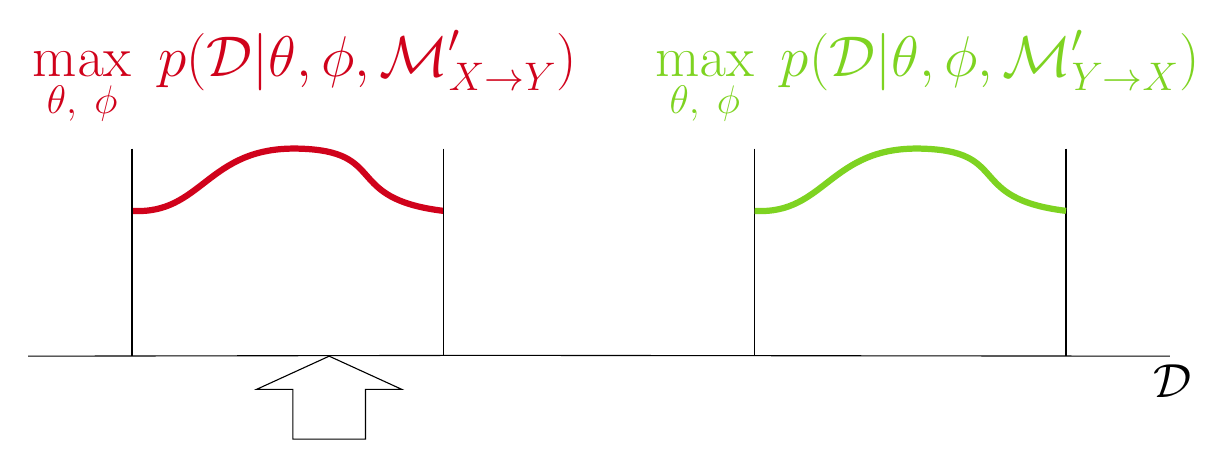
\begin{tikzpicture}[x=0.75pt,y=0.75pt,yscale=-1,xscale=1]
%uncomment if require: \path (0,300); %set diagram left start at 0, and has height of 300

%Straight Lines [id:da7493139746626474]
\draw    (50,180) -- (272,179.61) -- (600,180) ;
%Curve Lines [id:da8407783790065078]
\draw [color={rgb, 255:red, 208; green, 2; blue, 27 }  ,draw opacity=1 ][line width=2.25]    (100,110) .. controls (134,112) and (136,79) .. (180,80) .. controls (224,81) and (201,104) .. (250,110) ;
%Straight Lines [id:da43093054308218504]
\draw    (100,80) -- (100,180) ;
%Straight Lines [id:da43535242732295365]
\draw    (250,80) -- (250,180) ;
%Straight Lines [id:da45962598629903195]
\draw    (400,80) -- (400,180) ;
%Straight Lines [id:da42195523828352655]
\draw    (550,80) -- (550,180) ;
%Curve Lines [id:da3254916787493394]
\draw [color={rgb, 255:red, 126; green, 211; blue, 33 }  ,draw opacity=1 ][line width=2.25]    (400,110) .. controls (434,112) and (436,79) .. (480,80) .. controls (524,81) and (501,104) .. (550,110) ;
%Up Arrow [id:dp9268792588428787]
\draw   (160,196) -- (195,180) -- (230,196) -- (212.5,196) -- (212.5,220) -- (177.5,220) -- (177.5,196) -- cycle ;

% Text Node
\draw (591,183) node [anchor=north west][inner sep=0.75pt]  [font=\LARGE] [align=left] {$\displaystyle \mathcal{D}$};
% Text Node
\draw (51,22) node [anchor=north west][inner sep=0.75pt]  [font=\huge,color={rgb, 255:red, 208; green, 2; blue, 27 }  ,opacity=1 ] [align=left] {$\displaystyle \max_{\theta ,\ \phi } \ p(\mathcal{D} |\theta ,\phi ,\mathcal{M} '_{X\rightarrow Y})$};
% Text Node
\draw (351,22) node [anchor=north west][inner sep=0.75pt]  [font=\huge,color={rgb, 255:red, 126; green, 211; blue, 33 }  ,opacity=1 ] [align=left] {$\displaystyle \max_{\theta ,\ \phi } \ p(\mathcal{D} |\theta ,\phi ,\mathcal{M} '_{Y\rightarrow X})$};








\end{tikzpicture}

\end{document}
